\subsection{Process Flow Diagram}
\label{subsec:process_flow}
The diagram shown in Figure \ref{fig:process_flowchart} the different processes 
that the system will undergo once it has been deployed in the server.

% Process Flowchart
\begin{figure}[ht]
    \centering
    
\includegraphics[height=1\textheight]{./assets/Chapter_3/PFC/ProcessFlowchart.png}
    \caption{Full Overview of the Process Flow Diagram for the alamSYS}
    \label{fig:process_flowchart}
\end{figure}
\FloatBarrier

To better view and understand the flow of the processes, 
we can divide the discussions per components in the diagram.

\subsubsection{Scheduler}
\label{subsubsc:scheduler}
Using CRON, a Linux-based scheduler, a 
scheduled task is provided to the server running the system. Since, 
the system will be containerized in a Linux System, the scheduler will 
run once the instance of the Docker Engine is running on the server system, 
which can be of any operating system. Then, if the current date and time of 
the contained system matches the scheduled date and time from CRON, it will 
log that the scheduled task has started, otherwise, it will not do anything 
and will check again for the current date and time.
\hfill \\

The consequent processes in this process flow diagram will run after the 
scheduled task is initiated. Wherein the schedule task will run everyday from 
Mondays to Fridays, every 5:00 P.M. And the whole process can be seen in the 
Figure \ref{fig:process_flowchart_scheduler}.
% Process Flowchart (Scheduler)
\begin{figure}[ht]
    \centering
    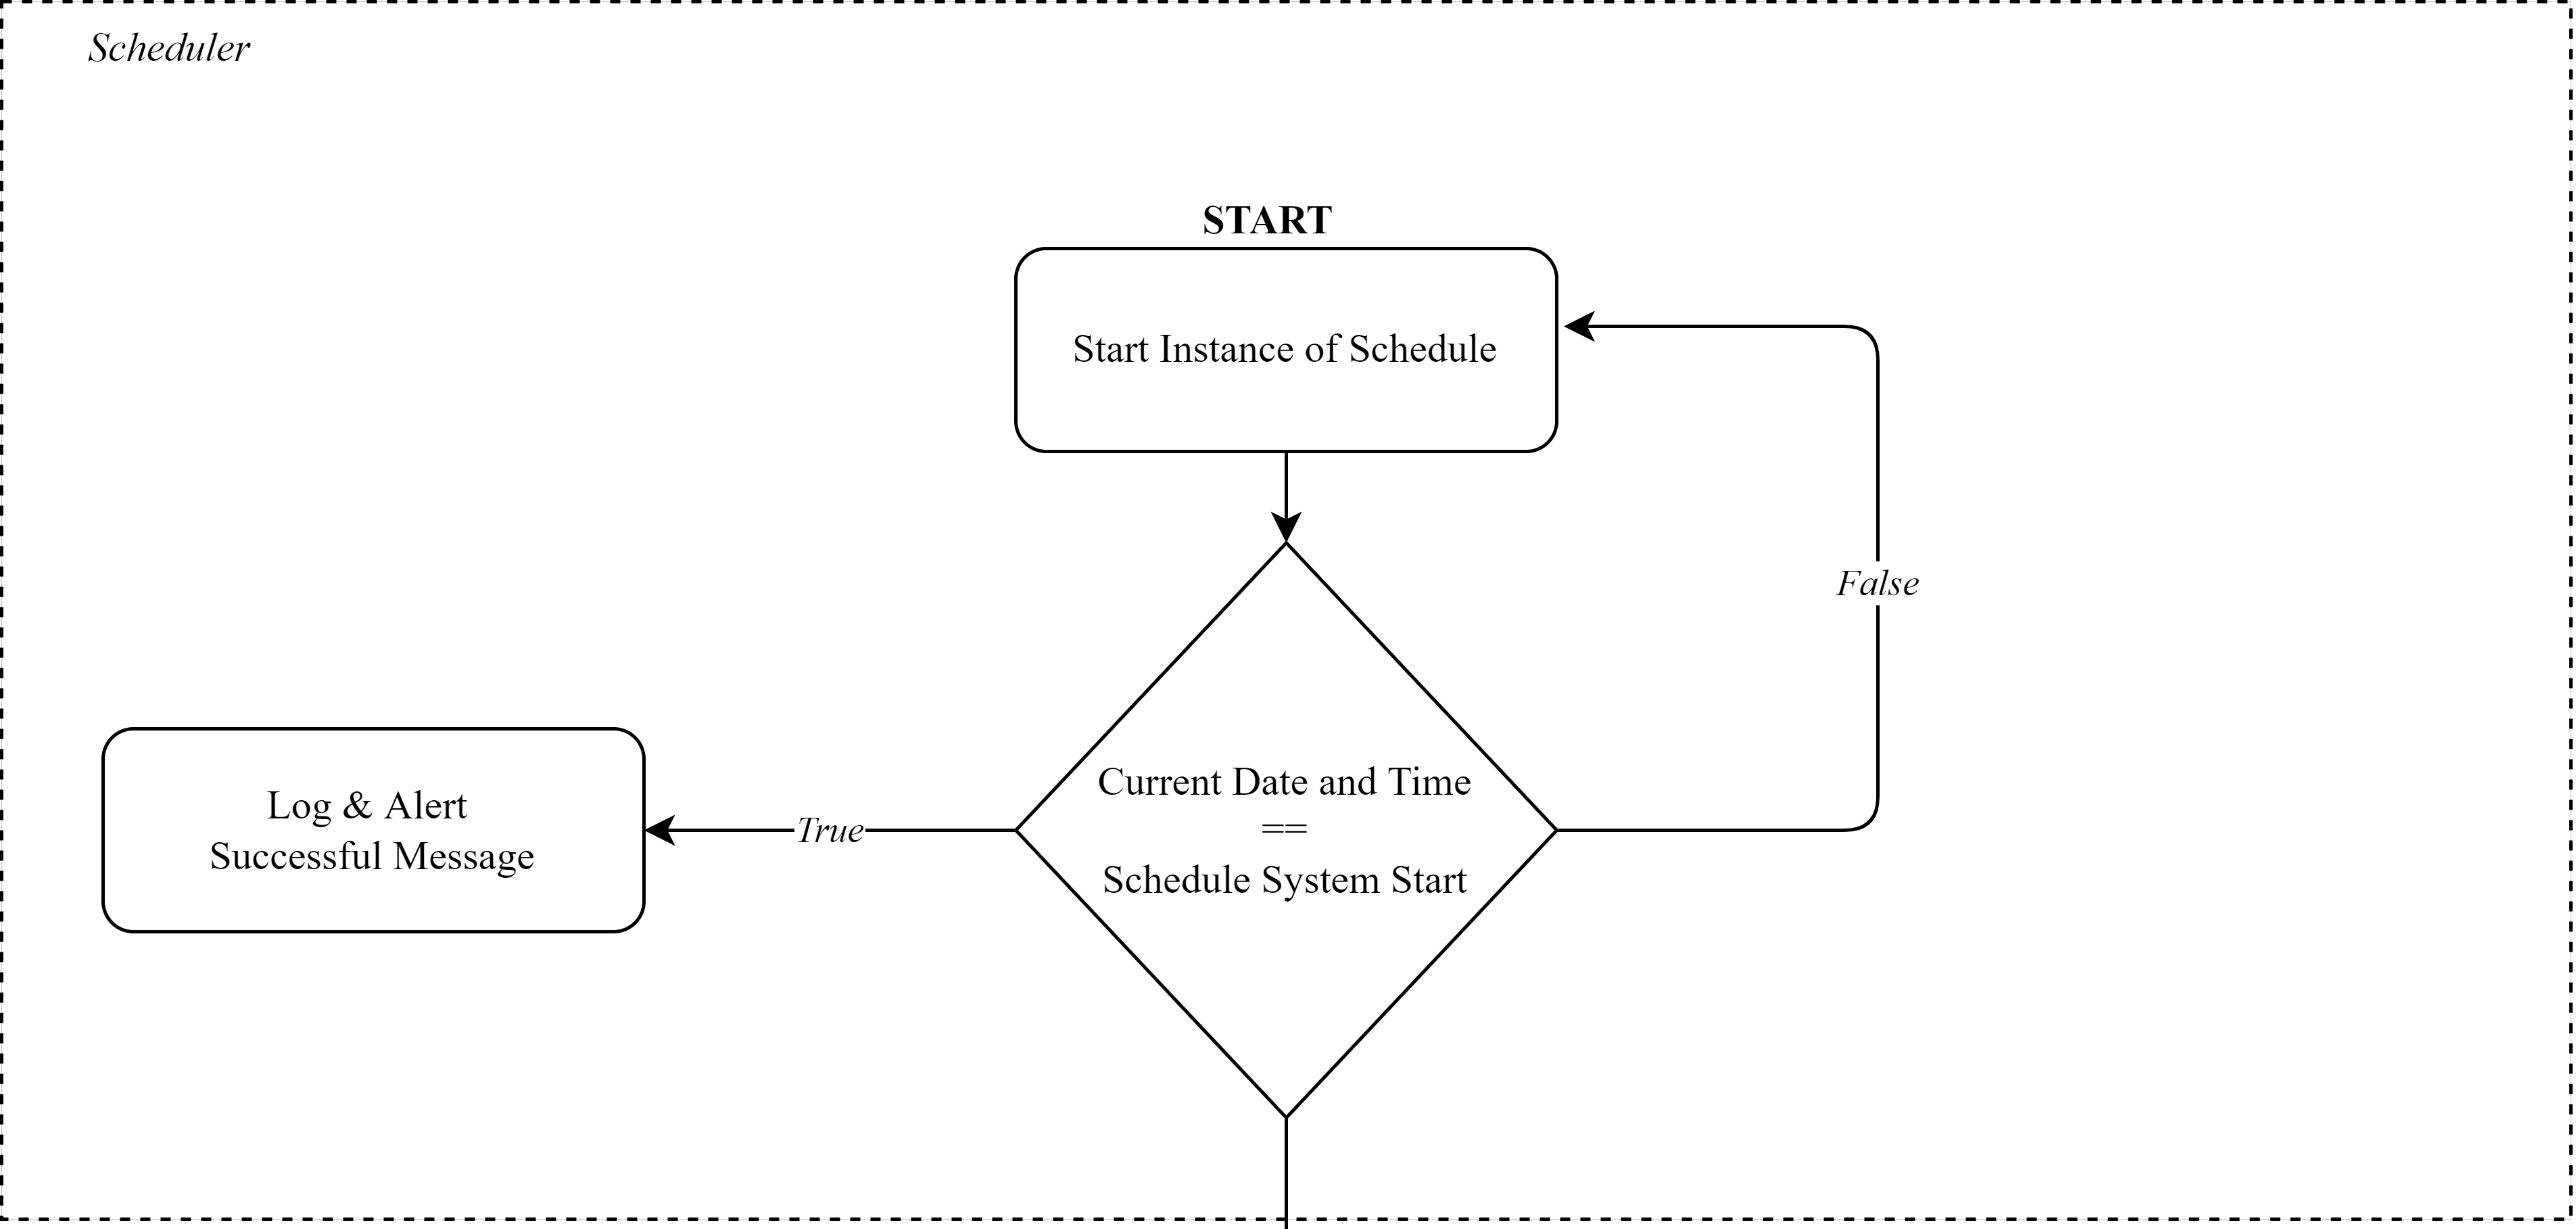
\includegraphics[width=1\textwidth]{./assets/Chapter_3/PFC/ProcessFlowchart_Scheduler.png}
    \caption{Overview of the Process Flow Diagram for the Scheduler}
    \label{fig:process_flowchart_scheduler}
\end{figure}
\FloatBarrier

\subsubsection{Data Collector}
\label{subsubsec:data_ollector}
This is the first task that the scheduled 
activity will do, which is simply to connect to the historical market 
data provider and collect the historical market data that is updated for 
the current date.
\hfill \\

Wherein, if the collection is successful, it will log that 
the system has successfully connected and collected the updated 
historical market data for that day and will proceed to use the 
collected data to the Machine Learning Model.
\hfill \\

Otherwise, it will log the error, and it will check the error message. 
Wherein, if the error message shows “Error 406” of “Payment Needed”, 
then the scheduled task will end in this section. This is also the reason why 
the end of each process ends in logging the activities of the system, so that 
the maintainers of the system can easily pin-point the problem to be fixed during 
the actual deployment of the alamSYS. Moreover, if the error is anything else, 
then the system will retry to collect the data for a maximum of five tries, and 
if it still encounters an error during the retry window, the session will also end.
\hfill \\

The flow of processes discussed above can be observed in Figure \ref{fig:process_flowchart_data_collector}.

% Process Flowchart (Data Collector)
\begin{figure}[ht]
    \centering
    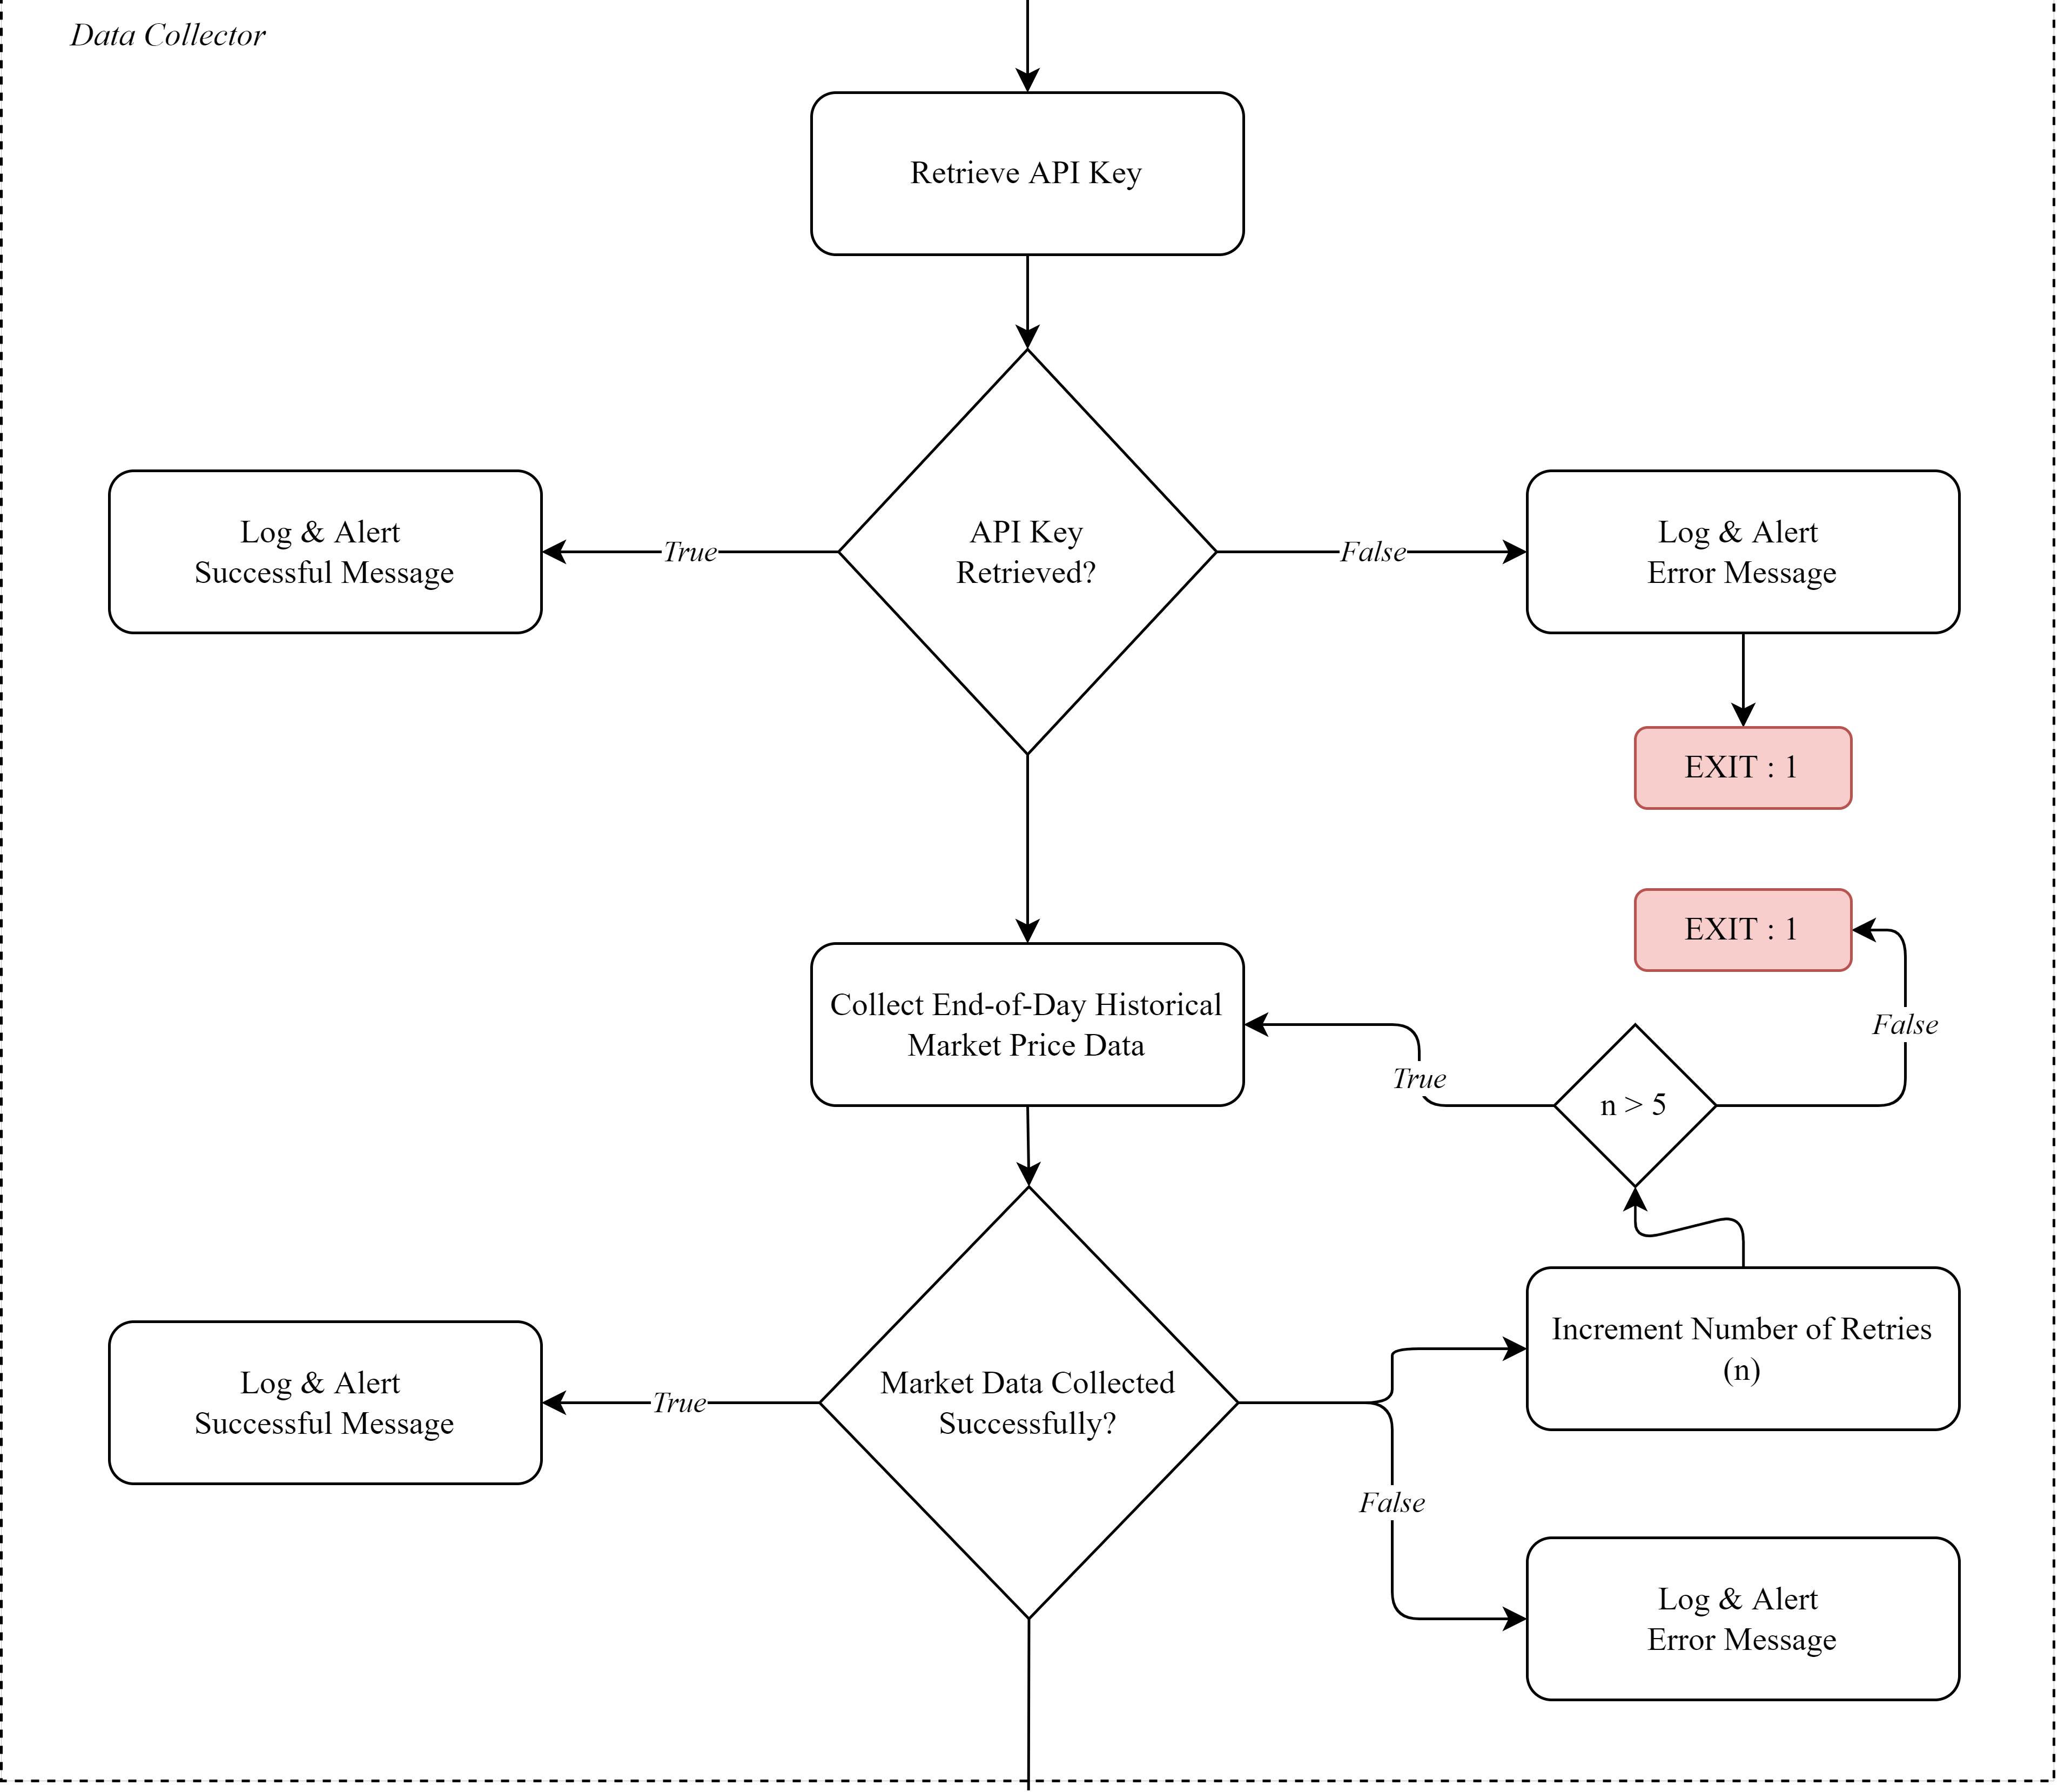
\includegraphics[width=1\textwidth]{./assets/Chapter_3/PFC/ProcessFlowchart_DataCollector.png}
    \caption{Overview of the Process Flow Diagram for the Data Collector}
    \label{fig:process_flowchart_data_collector}
\end{figure}
\FloatBarrier

\subsubsection{Machine Learning Model Application}
\label{subsubsec:ml_application}
In this process the developed machine learning model/algorithm will use the 
current historical market data collected to predict the future trend of the 
stock market and decide whether that stock should be bought or sold for 
the next market day.
\hfill \\

Wherein if the application of the machine learning model is successful, 
then the system will log the success of the operation and proceeds into 
updating the database.
\hfill \\

Otherwise, it will log the error, and will retry the operation for a 
maximum of five times. Once after the five retries is unsuccessful, 
then the system will end the session at this stage.
\hfill \\

The flow of processes discussed above can be 
observed in Figure \ref{fig:process_flowchart_ml_application}.

% Process Flowchart (Data Processor)
\begin{figure}[ht]
    \centering
    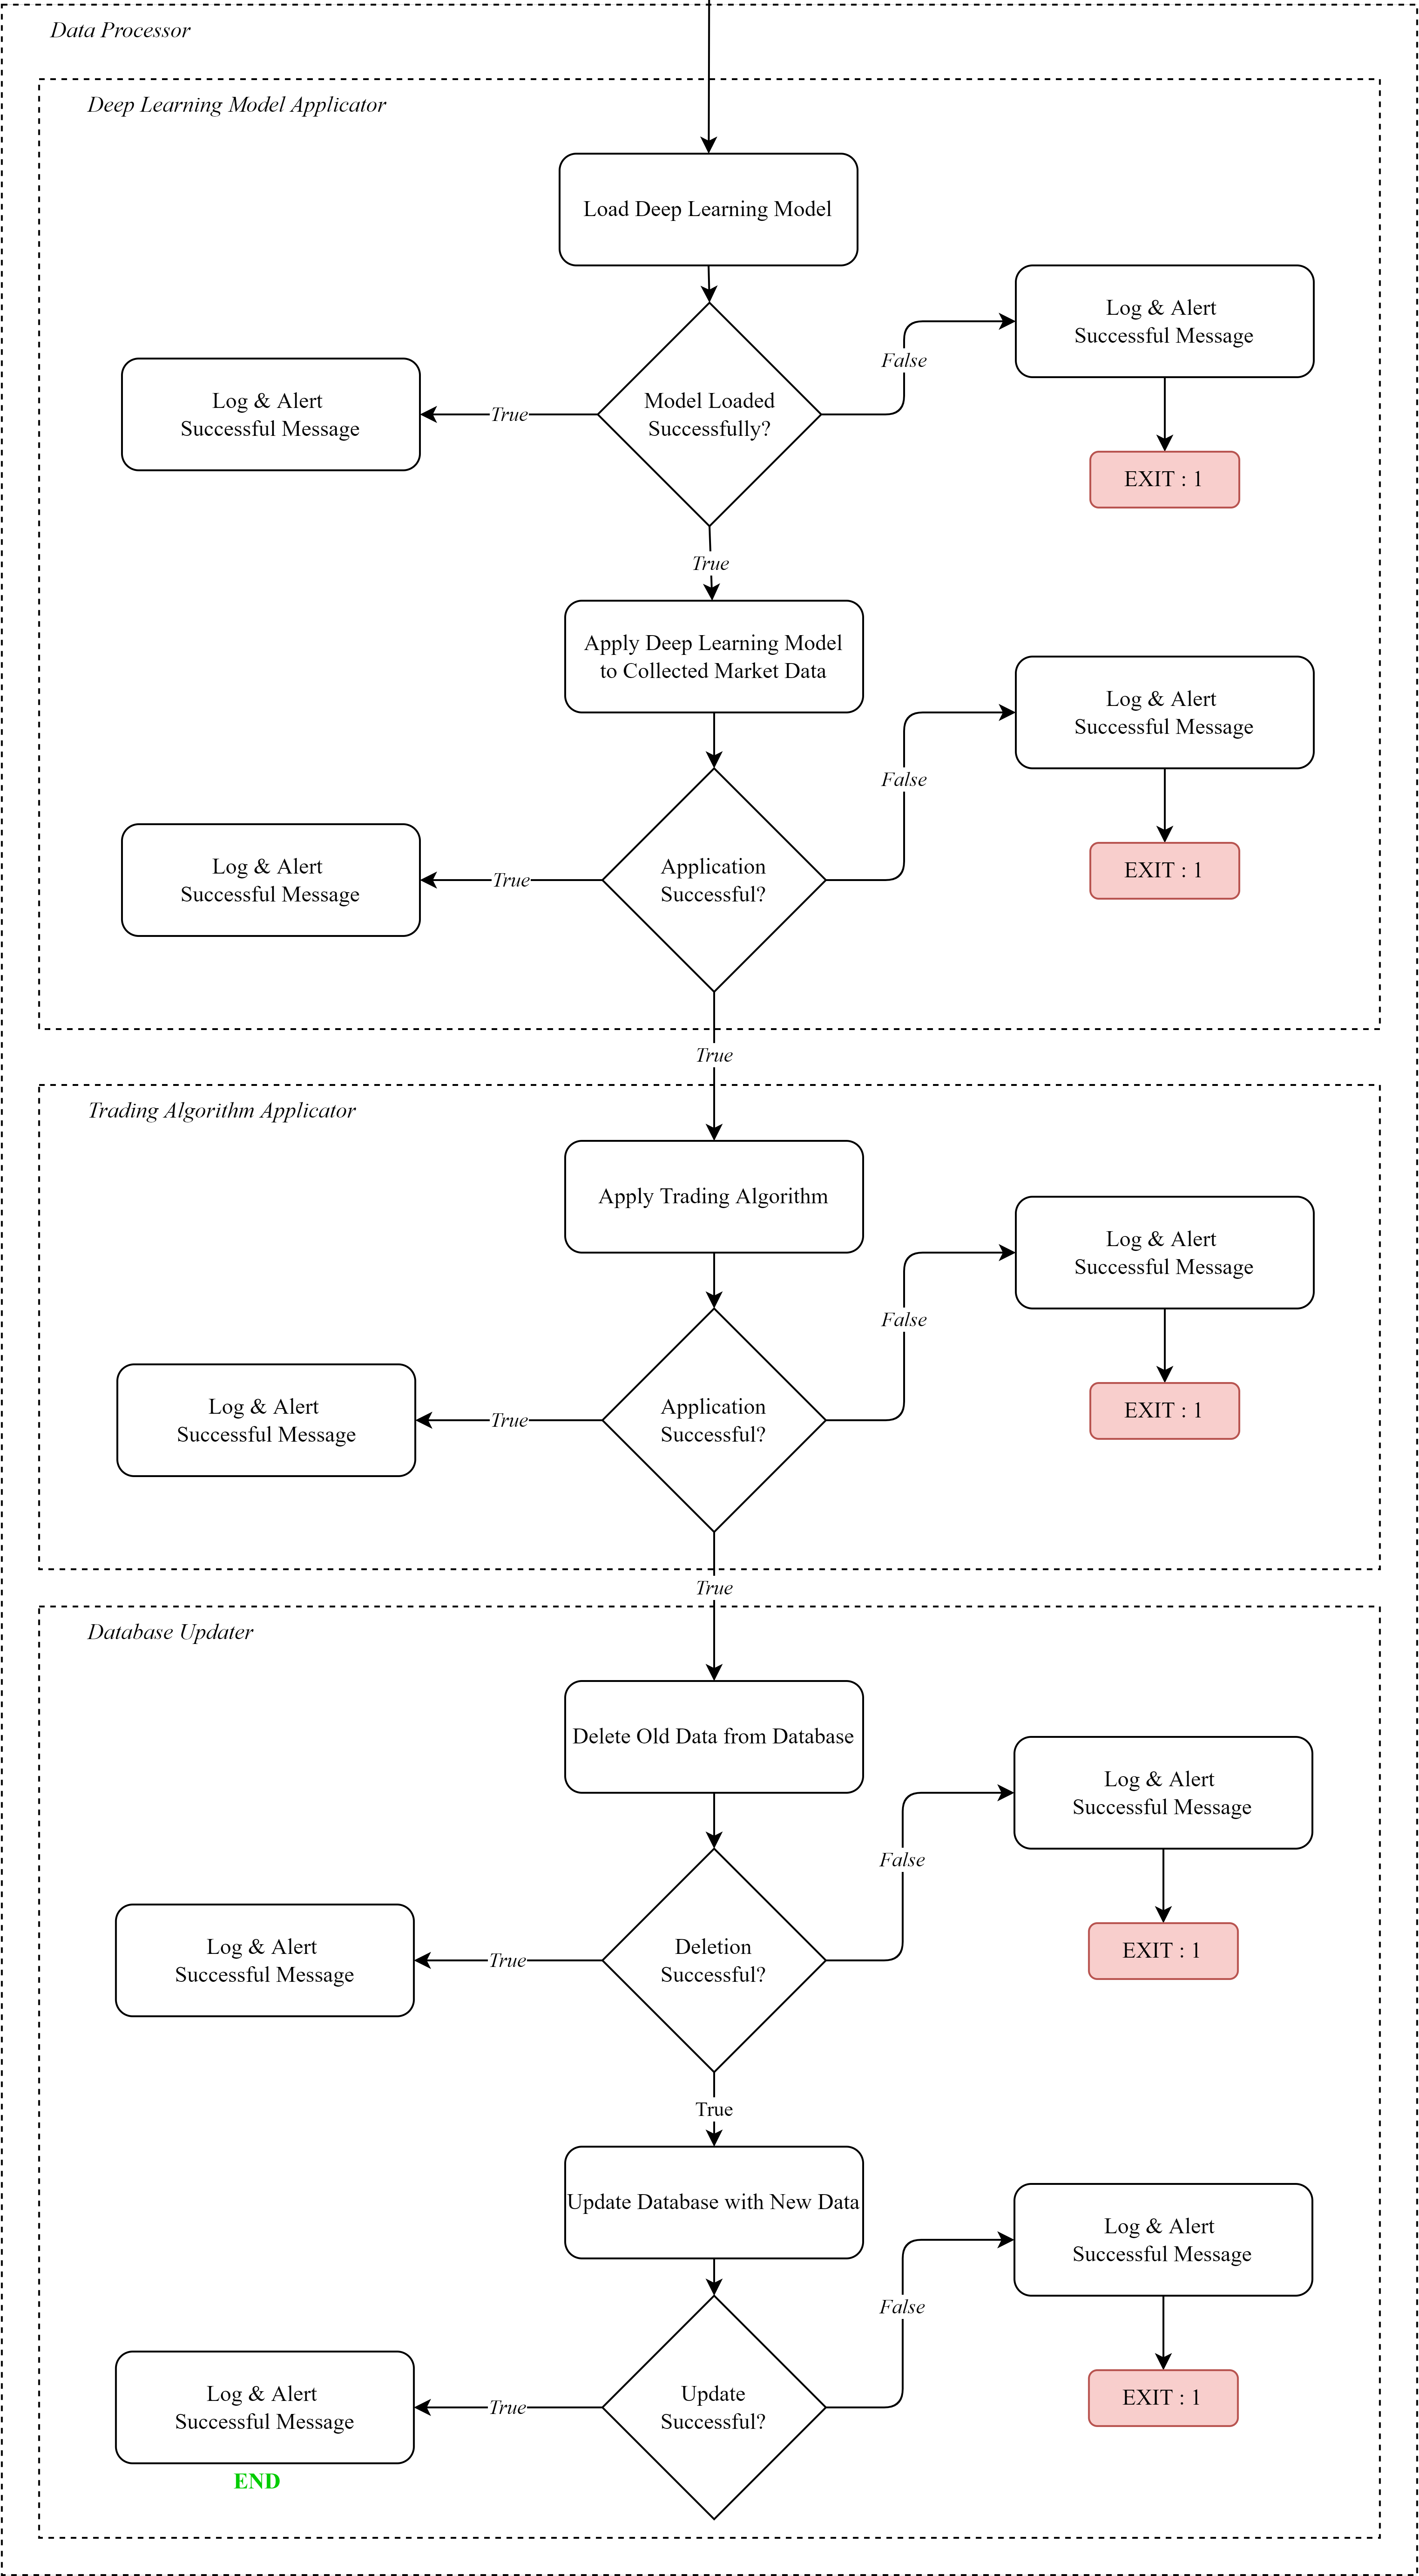
\includegraphics[height=1\textheight]{./assets/Chapter_3/PFC/ProcessFlowchart_DataProcessor.png}
    \caption{Overview of the Process Flow Diagram for Data Processor}
    \label{fig:process_flowchart_ml_application}
\end{figure}
\FloatBarrier

\subsubsection{Database Updater}
\label{subsubsec:db_updater}
This process flow will purge the old content of 
the database, and once successful it will update the database with the 
new documents created from the previous process.
\hfill \\

The flow of processes discussed above can be observed 
in Figure \ref{fig:process_flowchart_db_updater}.

% Process Flowchart (Data Processor - Deep Learning Model Applicator)
\begin{figure}[ht]
    \centering
    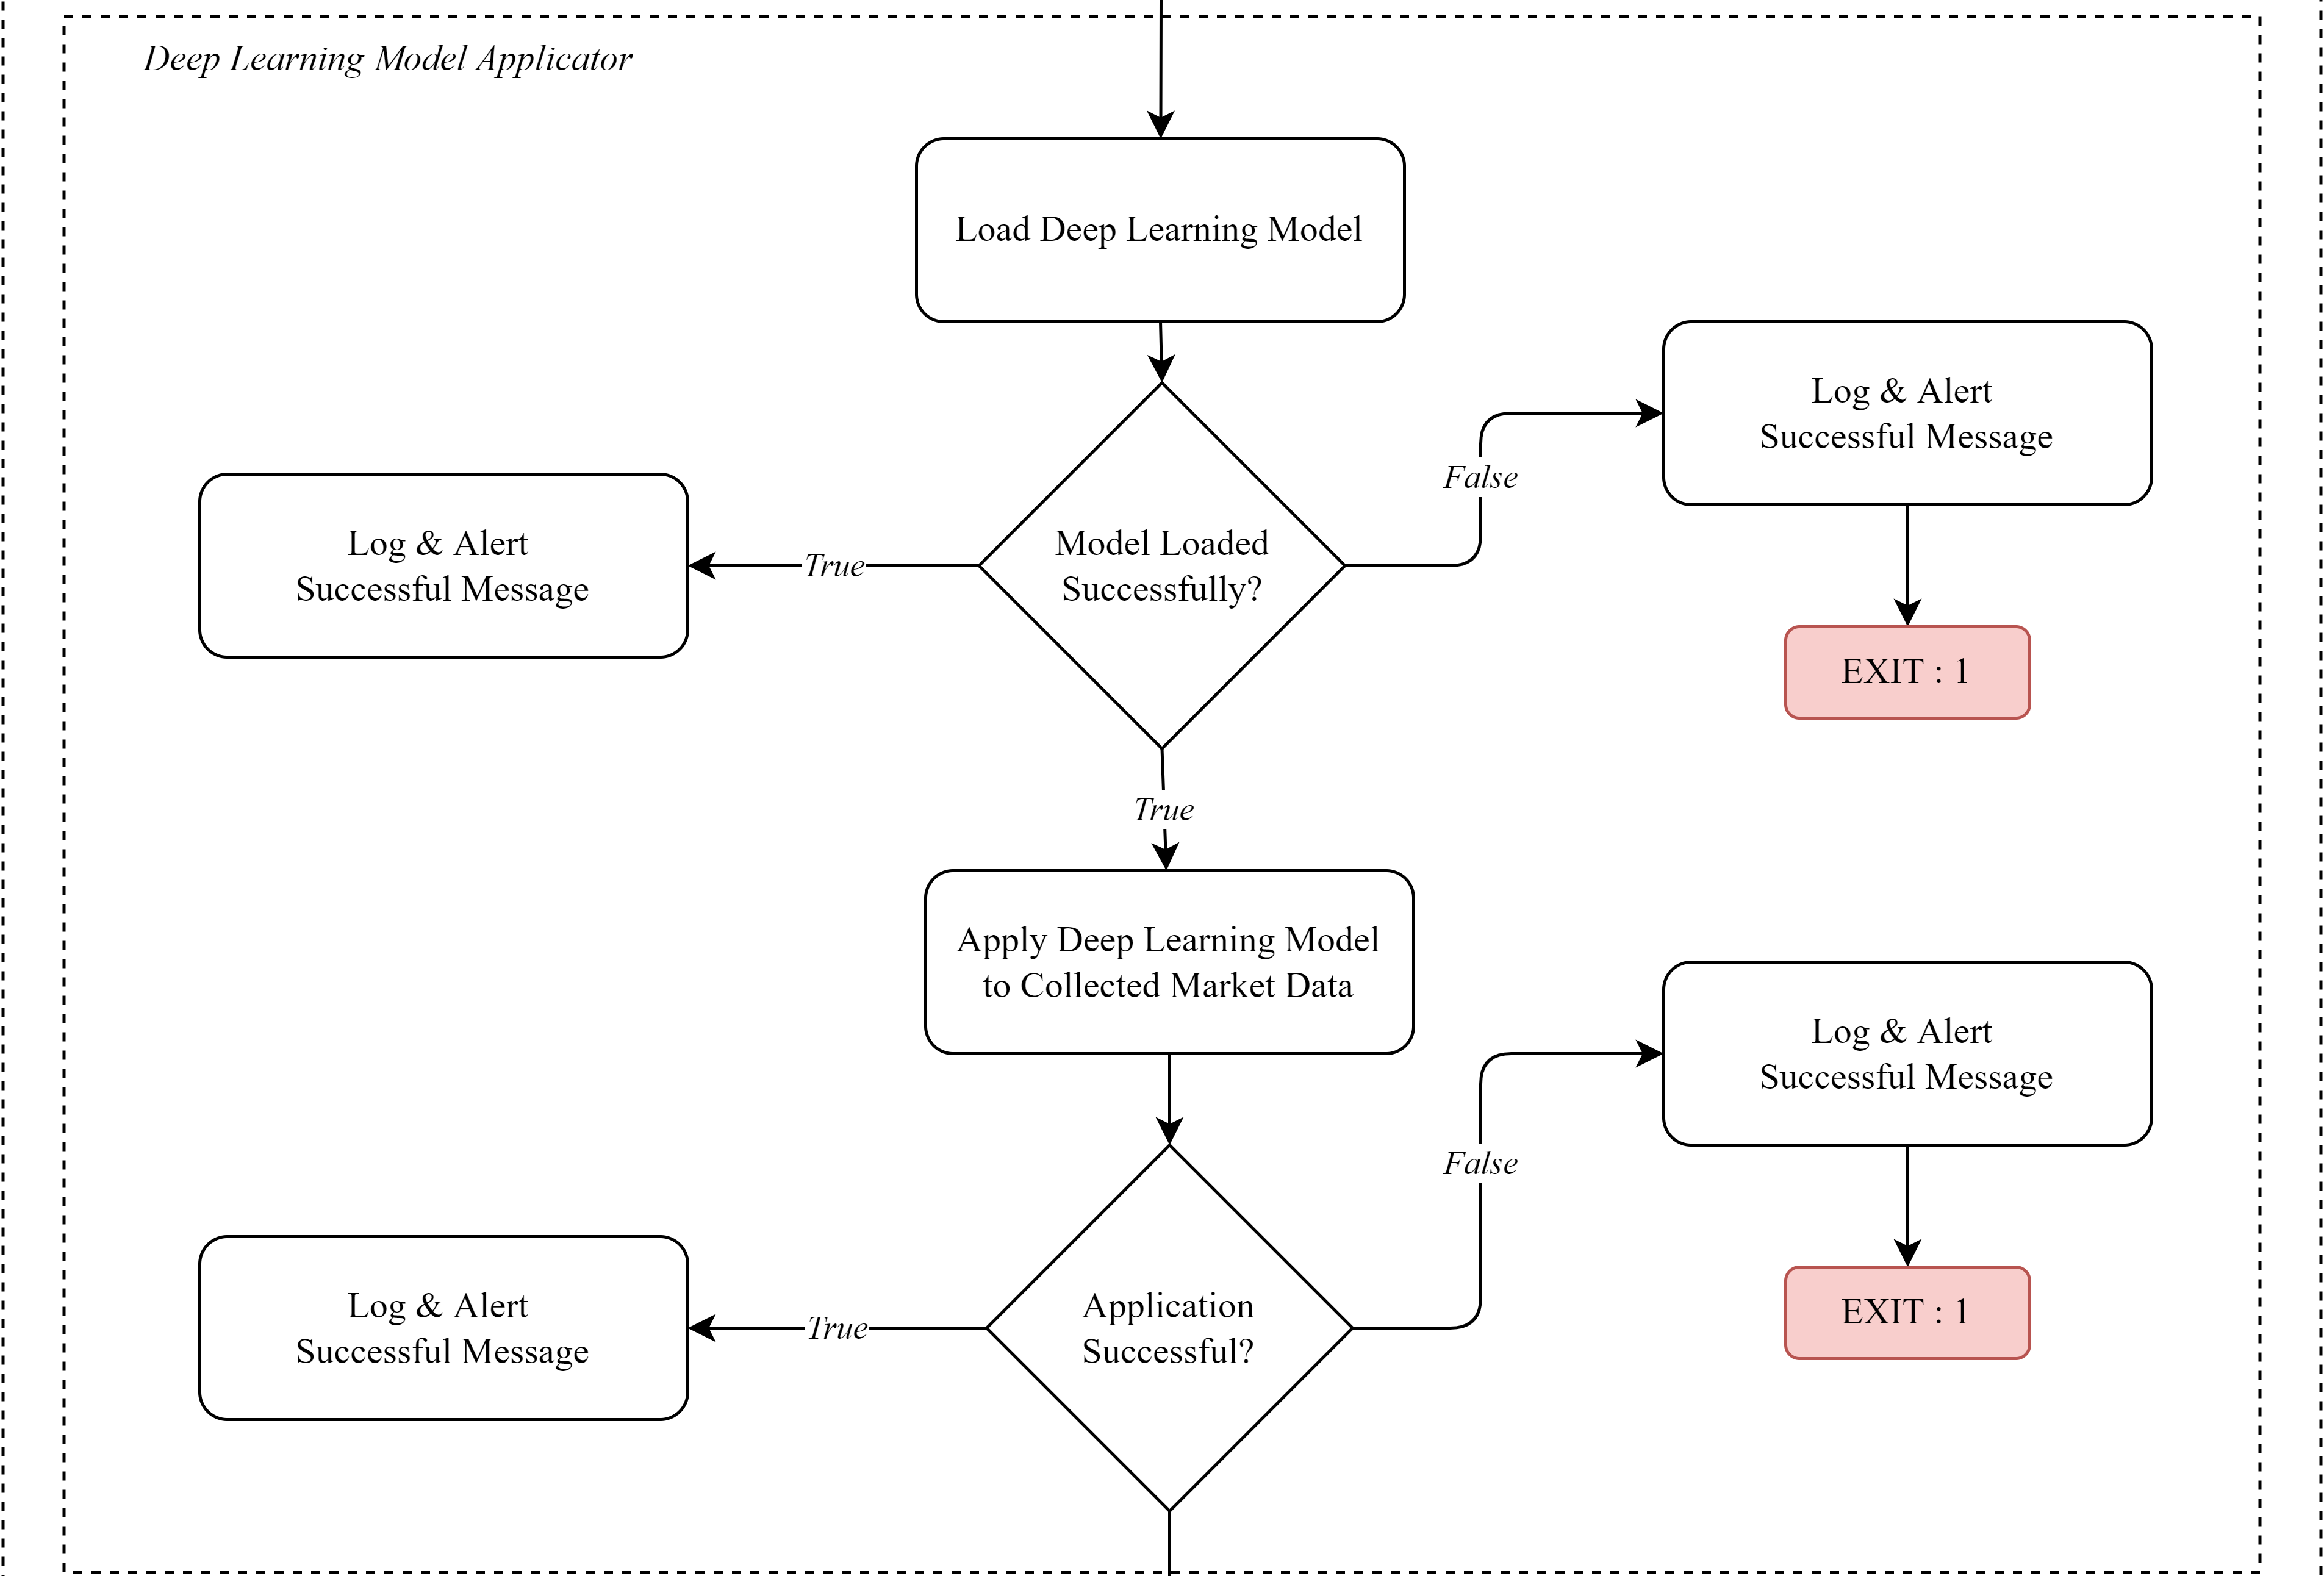
\includegraphics[width=1\textwidth]{./assets/Chapter_3/PFC/ProcessFlowchart_DataProcessor1.png}
    \caption{Overview of the Process Flow Diagram for the Deep Learning Model Applicator}
    \label{fig:process_flowchart_dp_model_applicator}
\end{figure}
\FloatBarrier

% Process Flowchart (Data Processor - Trading Algorithm Applicator)
\begin{figure}[ht]
    \centering
    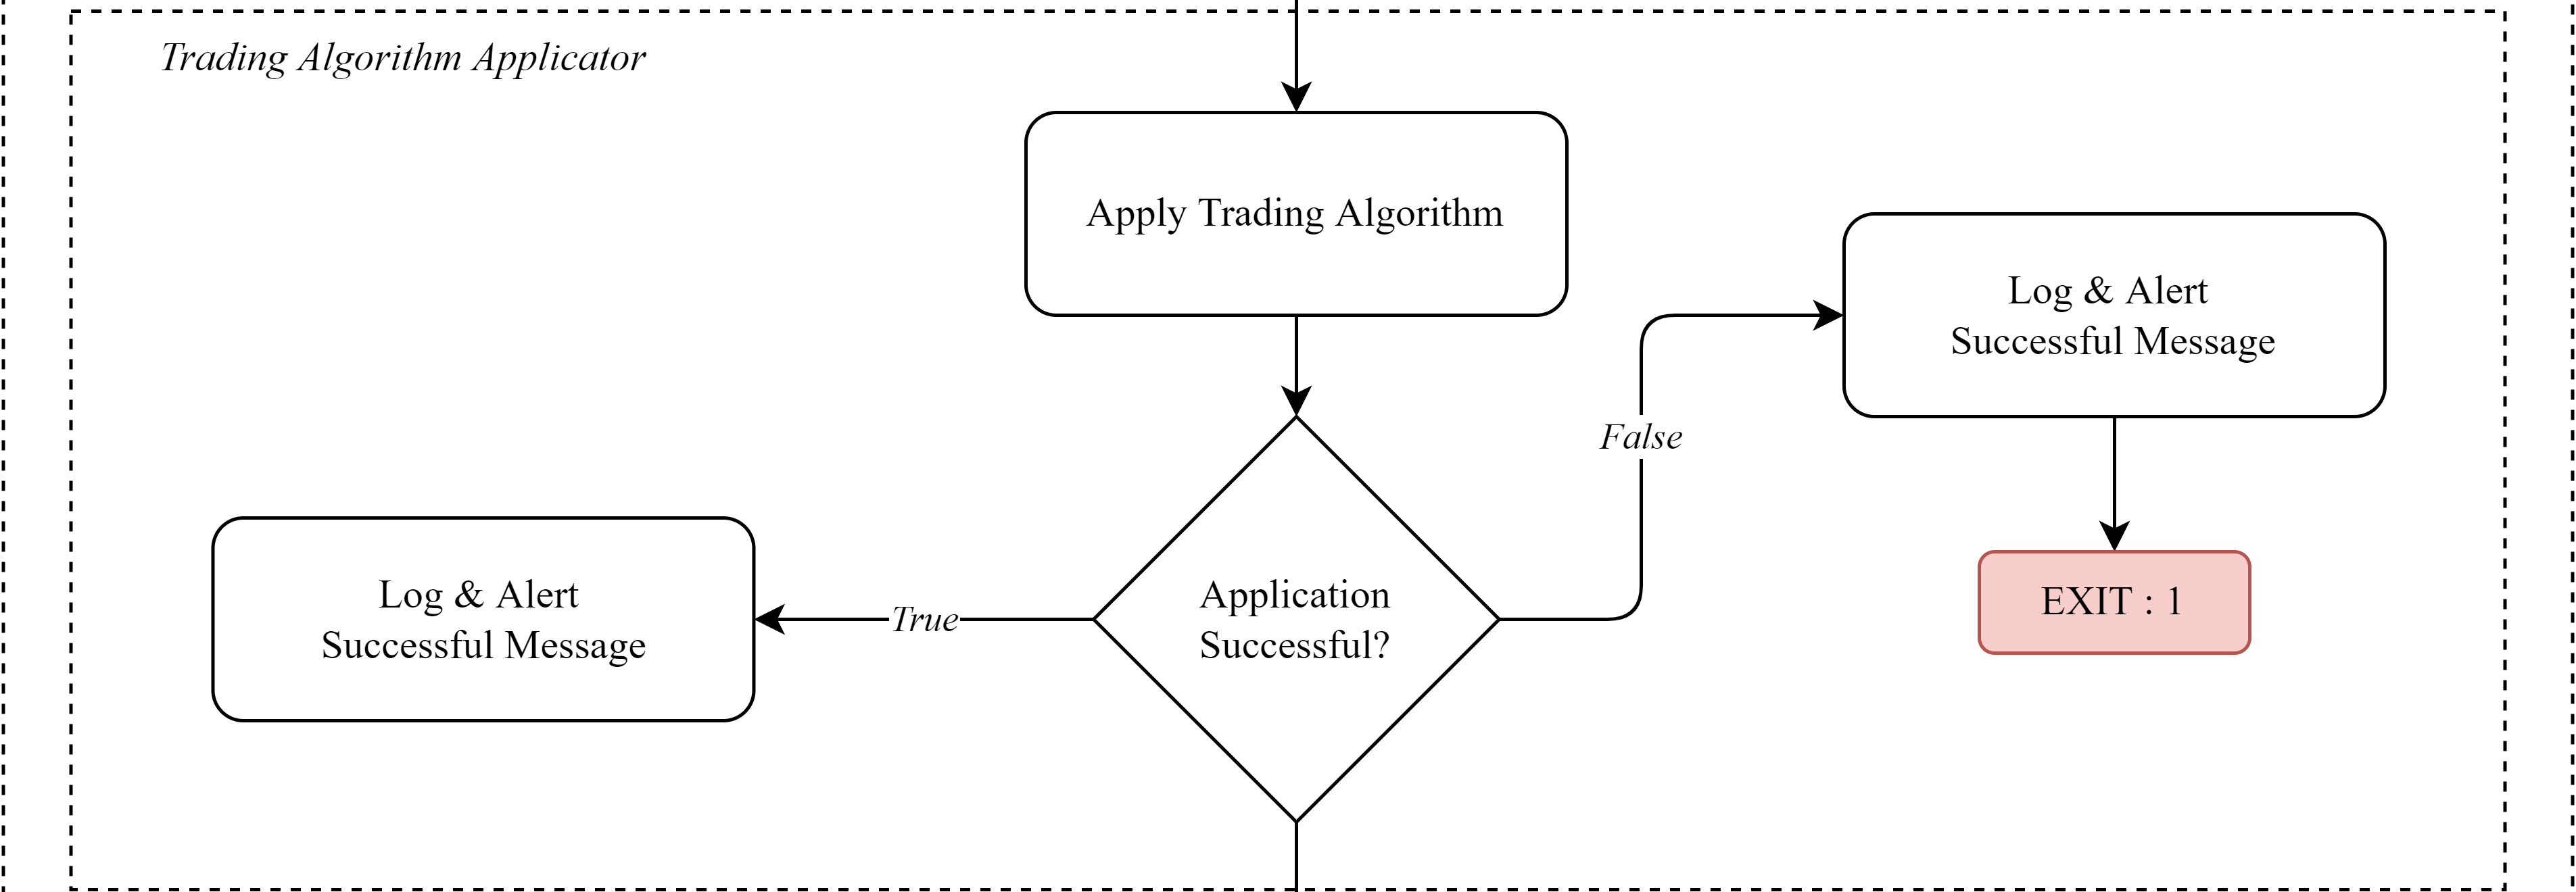
\includegraphics[width=1\textwidth]{./assets/Chapter_3/PFC/ProcessFlowchart_DataProcessor2.png}
    \caption{Overview of the Process Flow Diagram for the Trading Algorithm Applicator}
    \label{fig:process_flowchart_dp_trad_algo_applicator}
\end{figure}
\FloatBarrier

% Process Flowchart (Data Processor-Database Updater)
\begin{figure}[ht]
    \centering
    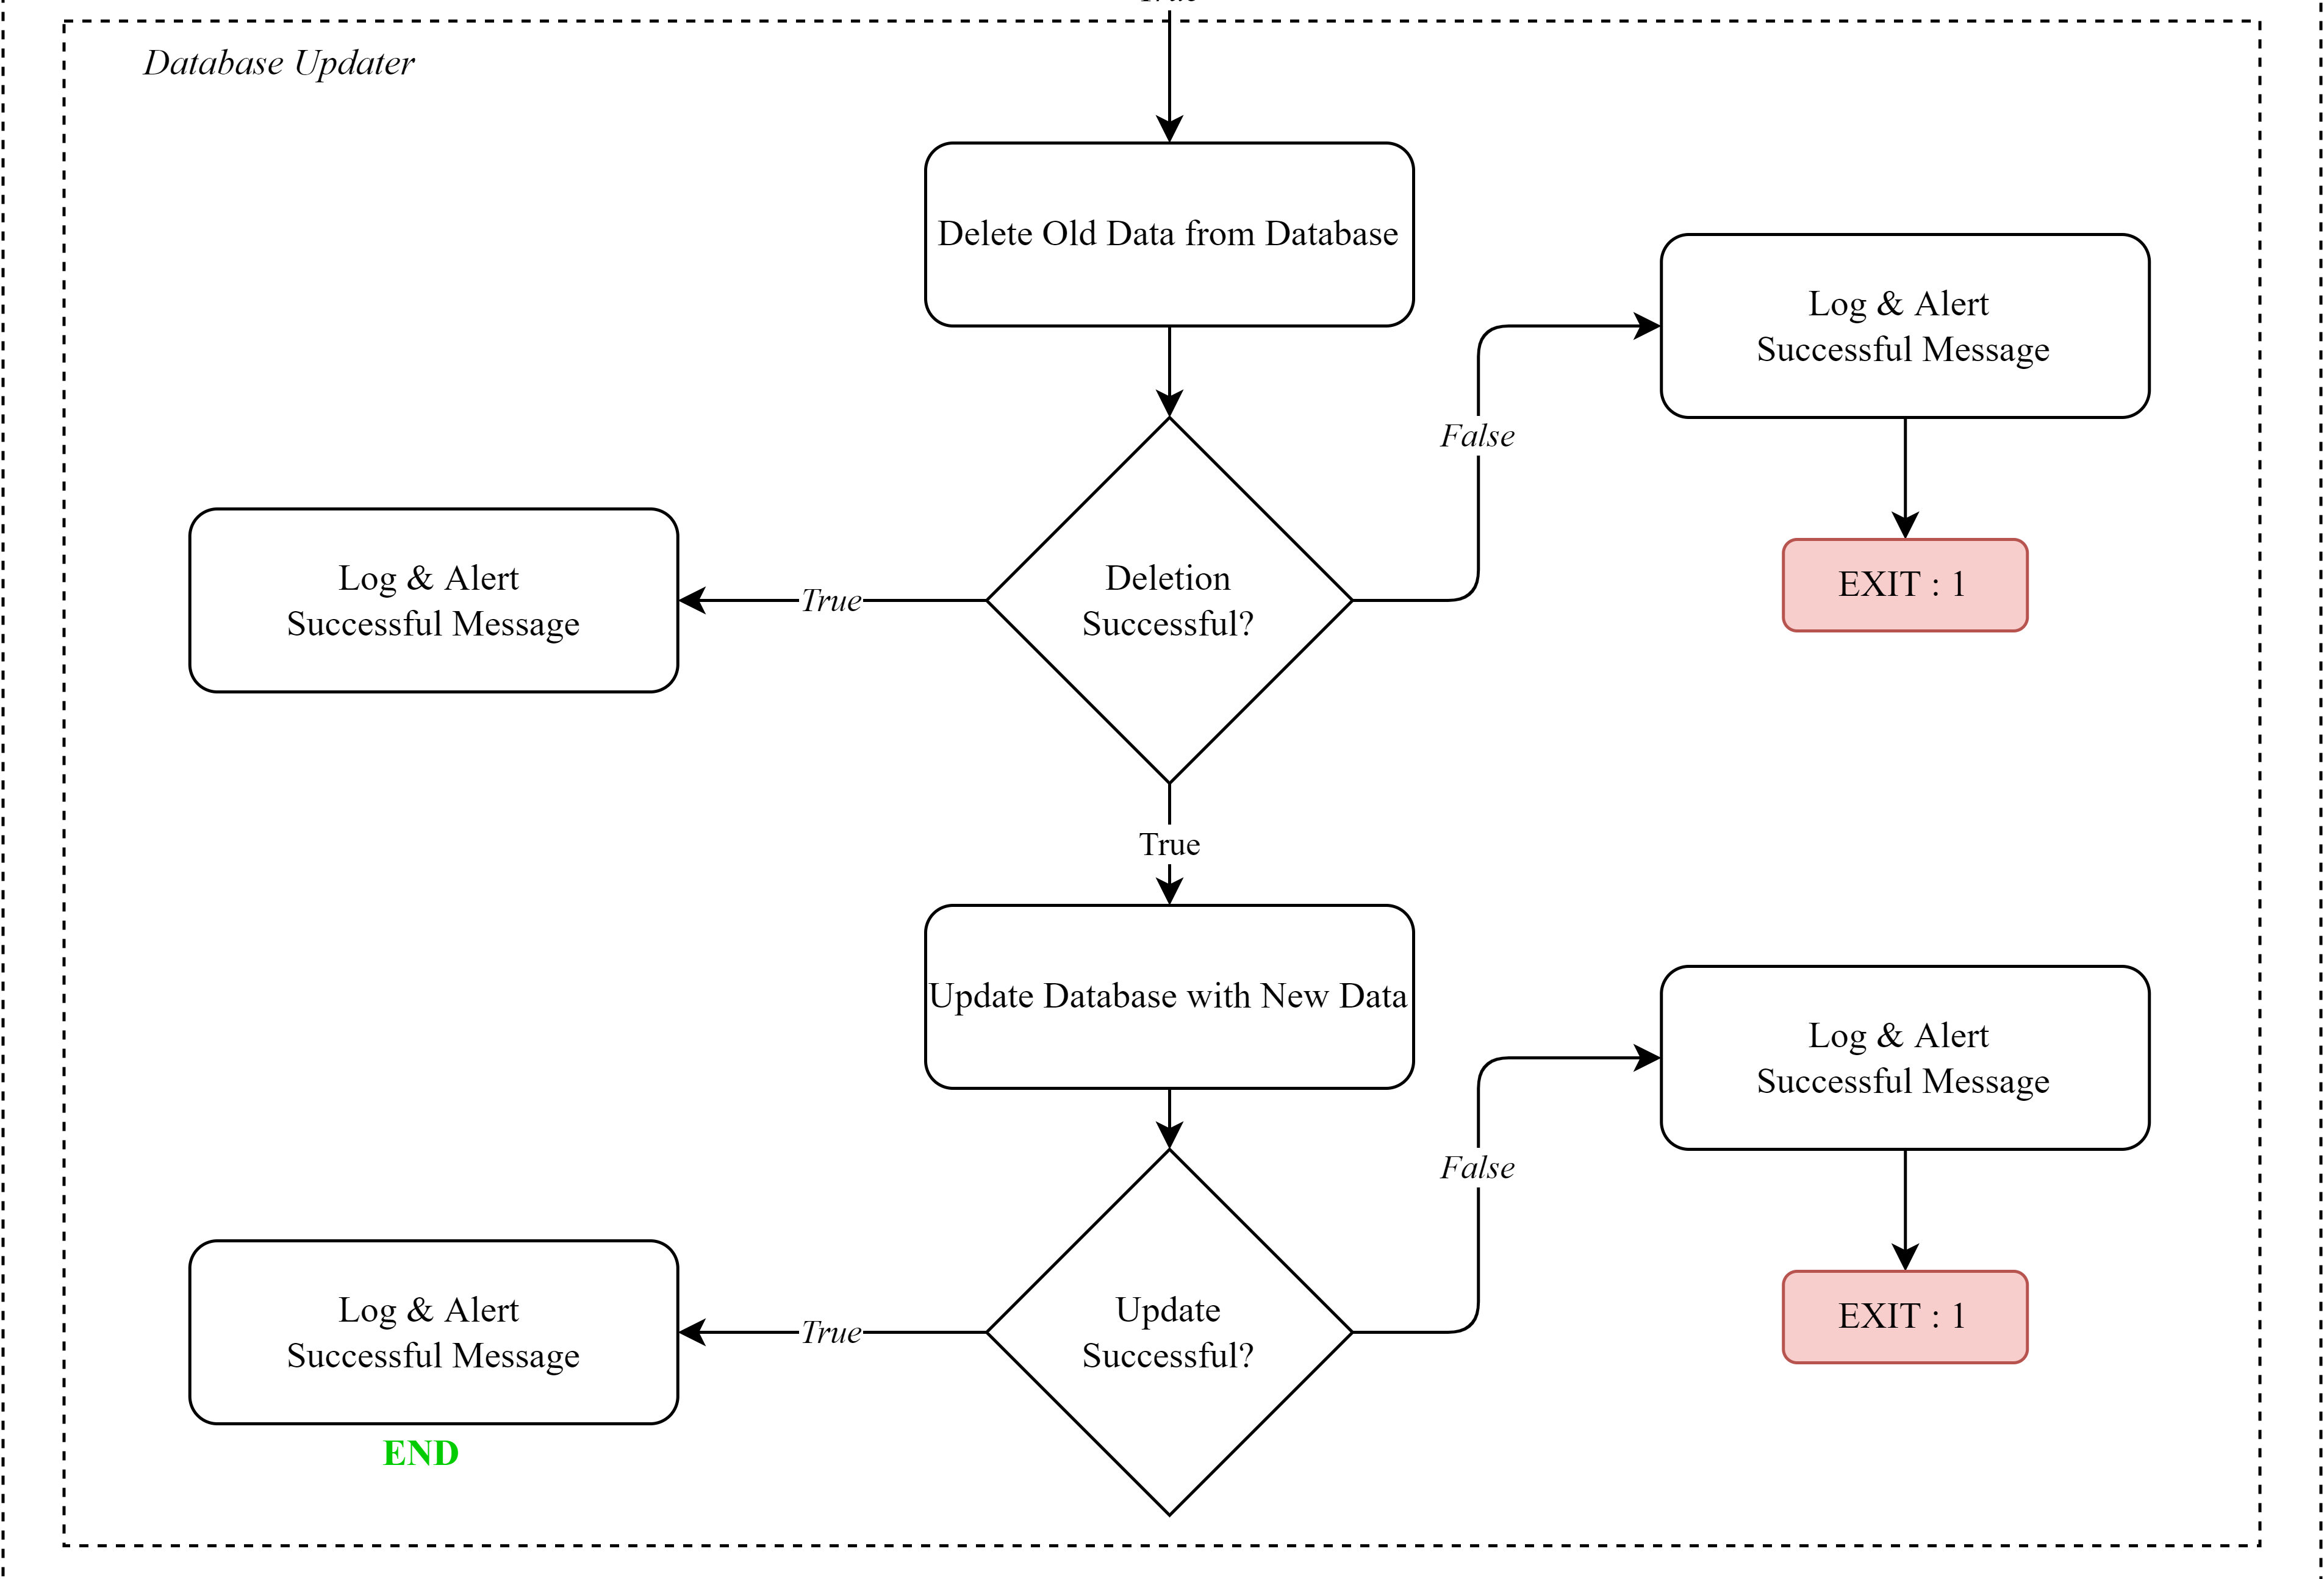
\includegraphics[width=1\textwidth]{./assets/Chapter_3/PFC/ProcessFlowchart_DataProcessor3.png}
    \caption{Overview of the Process Flow Diagram for the Database Updater}
    \label{fig:process_flowchart_db_updater}
\end{figure}
\FloatBarrier